\documentclass[aip,jap,reprint]{revtex4-2}
\usepackage{graphicx}
\graphicspath{{figures/}}
\usepackage{hyperref}
\usepackage{microtype}
\usepackage{xcolor}
\hypersetup{hidelinks,pdftitle={AgenticMM: A Material-Centered Multi-Agent Architecture for Scalable First-Principles Materials Modeling},pdfsubject={Material-centered multi-agent execution of structured prompt-based skills},pdfkeywords={AgenticMM, agentic AI, multi-agent systems, first-principles materials modeling, structured prompts, scientific workflows}}

\begin{document}

\title{AgenticMM: A Material-Centered Multi-Agent Architecture for Scalable First-Principles Materials Modeling}

\maketitle
\setcounter{dbltopnumber}{1}

\section{Introduction}

We introduce AgenticMM, a material-centered multi-agent architecture for scalable first-principles materials modeling. For each material, AgenticMM assigns one persistent agent that owns the complete workflow and retains material-specific context and execution history. A persistent coordinator agent allocates shared resources across dependency-ready tasks, mediates communication, routes unresolved scientific questions to the researcher, and tracks campaign-level completion. AgenticMM is designed to incorporate reusable, prompt-based skills as modular definitions of scientific workflows.\cite{atomisticskills,defectskills} We refer to these supplied skills as MatterSkills.

\section{Architecture and design principles}

As shown in Fig.~\ref{fig:agenticmm_architecture}, AgenticMM organizes the campaign around material-centered ownership. Throughout the campaign, each material agent owns its material's workflow and scientific context, while the coordinator manages campaign-wide information, shared resources, and communication. A campaign involving $N$ materials has exactly one coordinator role and one material-agent role per material, with no additional agent roles or layers. Supplied MatterSkills and researcher inputs provide the scientific guidance for the campaign. The design principles are detailed below.

\begin{figure*}[t]
  \centering
  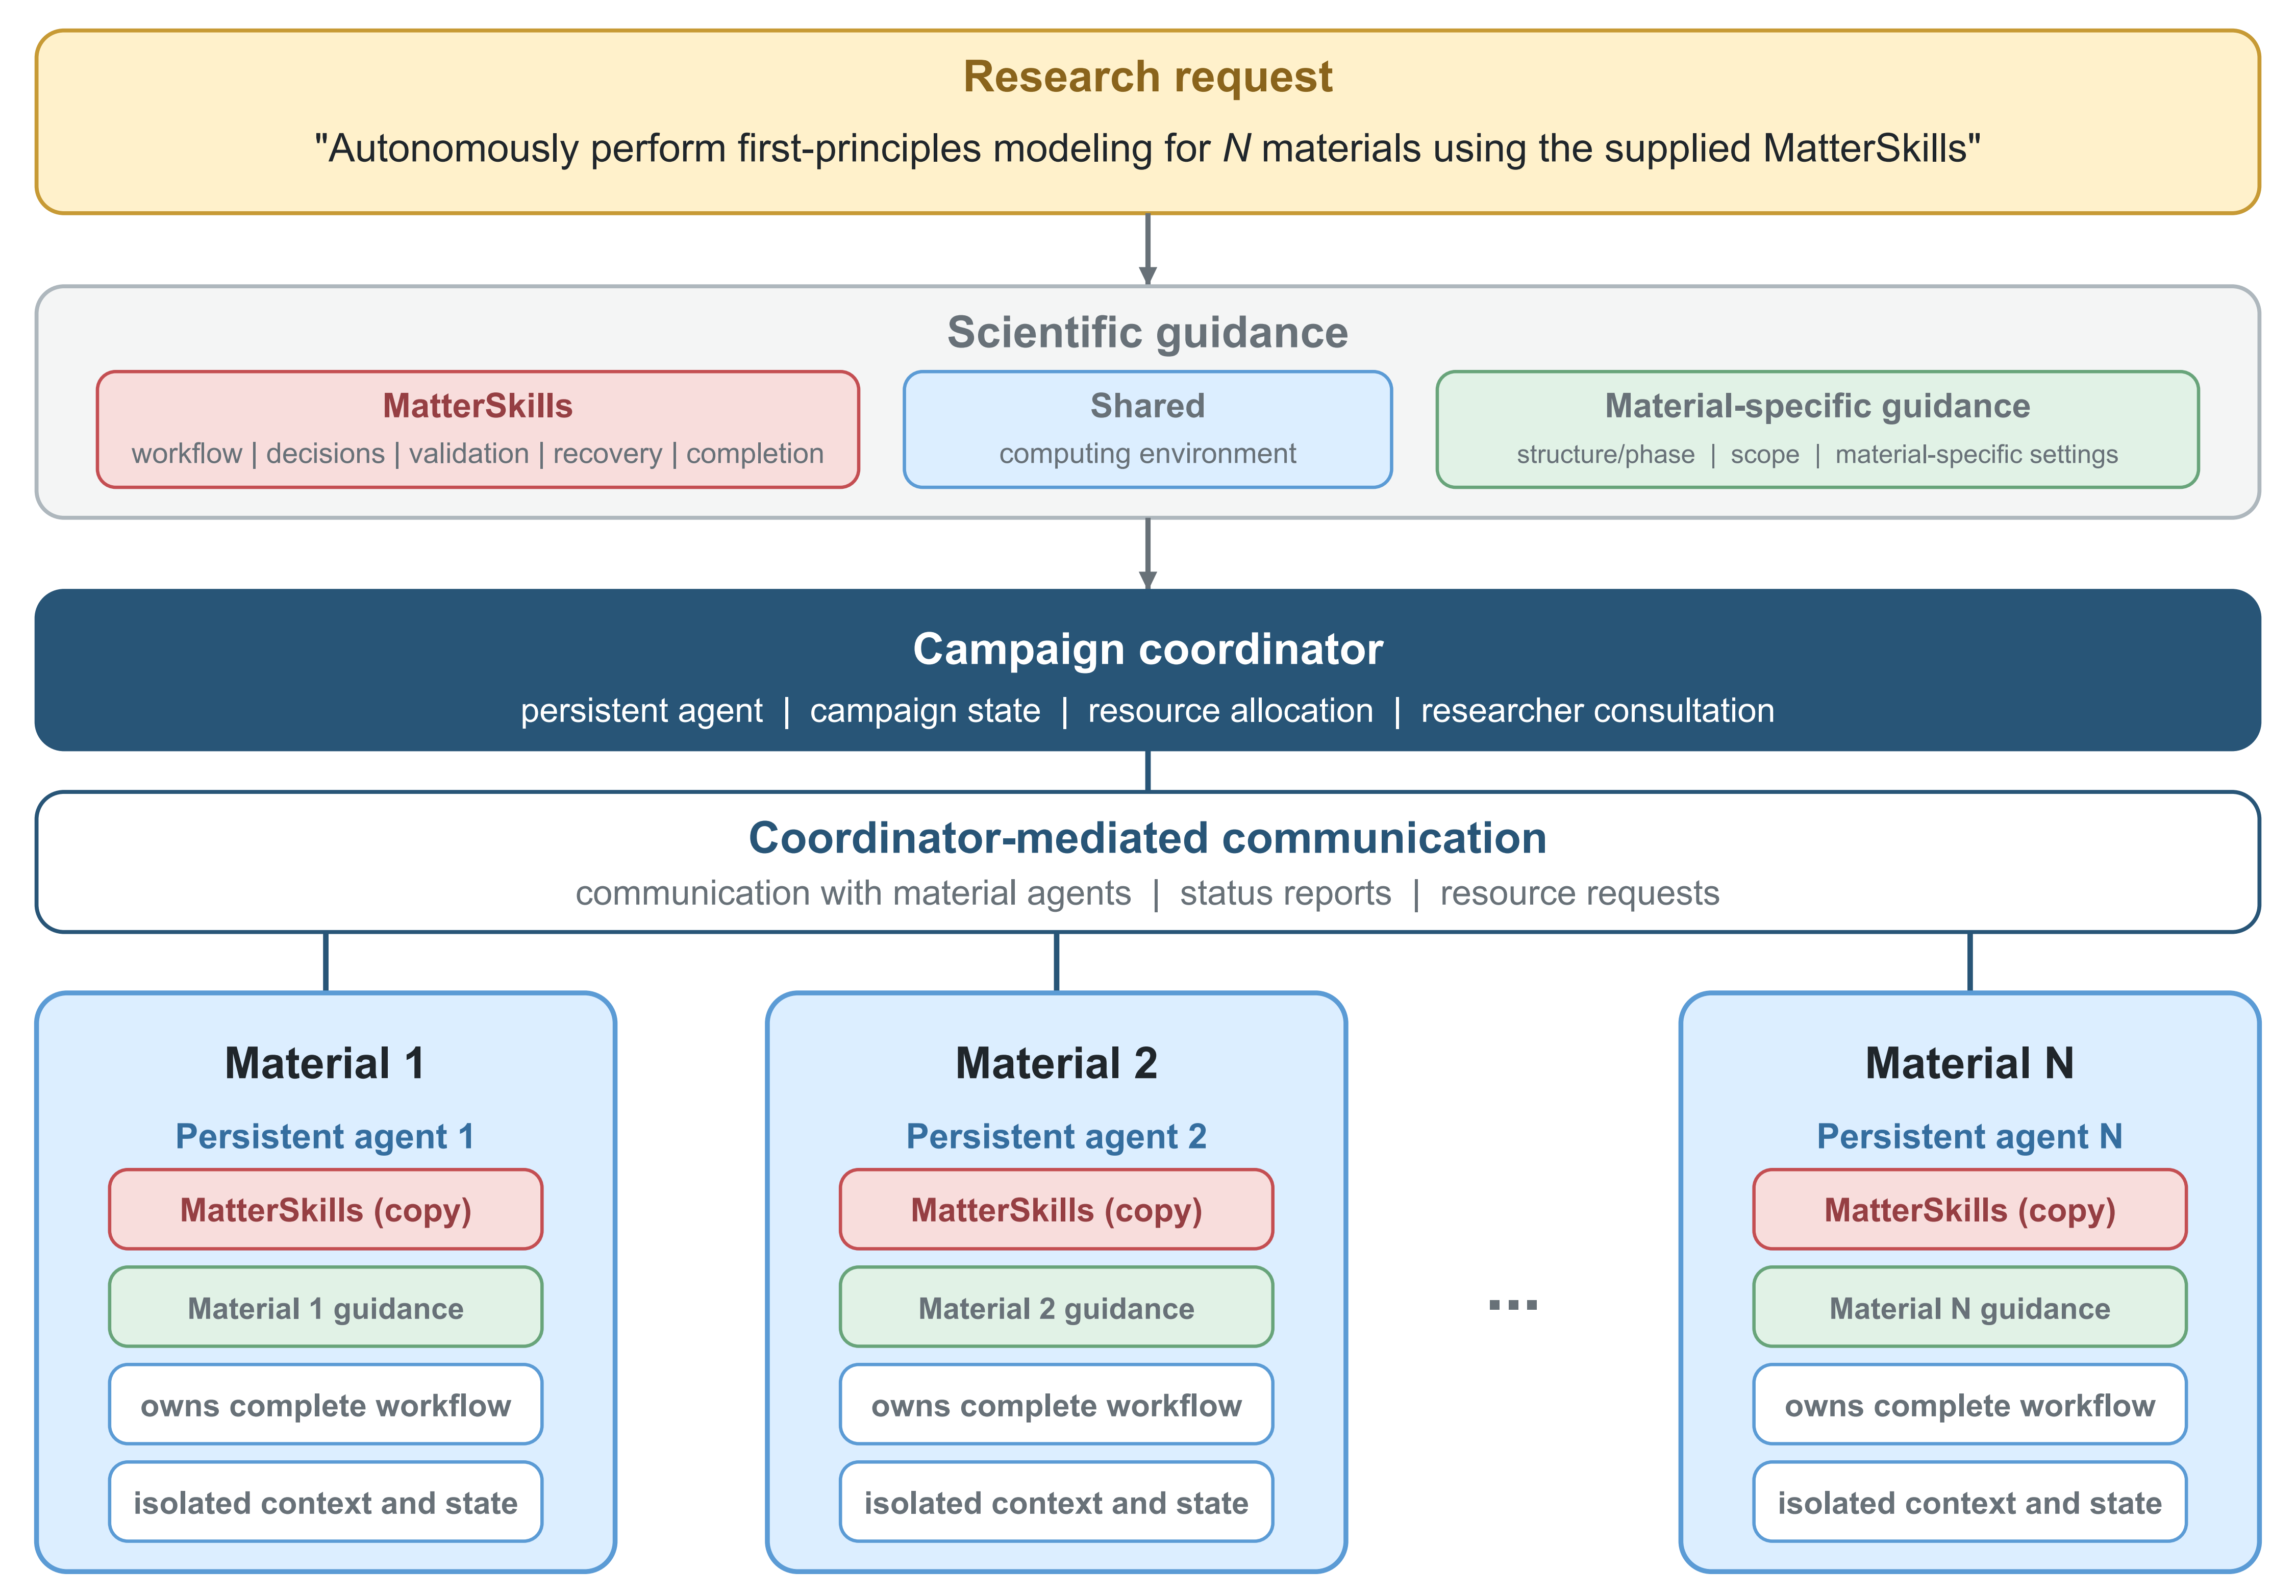
\includegraphics[width=0.92\textwidth]{figure_1.png}
  \caption{Architecture of AgenticMM. Supplied MatterSkills provide the primary scientific guidance, while researcher inputs define the campaign objective, shared computing environment, and scope and requirements for each material. A persistent coordinator agent distributes the applicable guidance, manages campaign state and shared resources, and mediates communication. Each persistent material agent receives the pinned MatterSkills release and relevant material-specific guidance, owns the complete MatterSkills-defined workflow, and maintains isolated context and state for one material. Material agents communicate only with the coordinator and do not share material-specific information with one another.}
  \label{fig:agenticmm_architecture}
\end{figure*}

\noindent\textbf{Material-centered ownership.} For each material, one persistent agent is the sole owner of the complete MatterSkills-defined workflow and its authoritative material-specific state, including inputs, calculation settings, intermediate results, decisions, and records of execution, failures, interruptions, and recovery actions. Material-specific information is not shared with other material agents. This ownership boundary reduces the risk of cross-material context mixing and allows materials to progress independently and at different rates.

\noindent\textbf{Campaign-level coordination.} The campaign coordinator agent maintains campaign-level state and coordinates activities across materials. It records the campaign objective, material-agent assignments and reassignments, shared settings and decisions, compact status reports, resource allocations, and completion state. During campaign setup, it assigns each material to one persistent agent and distributes the pinned MatterSkills and relevant researcher inputs, including the shared computing environment and the scientific scope and requirements for that material. During execution, it allocates shared resources based on material agents' reports of task readiness and resource needs, tracks progress toward campaign completion, and routes unresolved scientific questions to the researcher. Material agents communicate only with the coordinator agent and do not exchange material-specific information with one another. The coordinator agent neither performs material-level calculations nor aggregates detailed scientific state across materials. The coordinator and material-agent roles are persistent logical roles whose authoritative states survive interruptions and enable resumption or reassignment. Persistence does not require indefinitely running conversations.

\noindent\textbf{Separation between scientific workflows and the multi-agent architecture.} Supplied MatterSkills define the scientific workflow through instructions, decision rules, validation criteria, recovery procedures, and completion criteria. During campaign setup, researcher inputs define the overall campaign objective, shared computing environment, and the scientific scope and requirements for each material. This guidance is supplied independently of AgenticMM. The architecture organizes agents, communication, resources, and persistent execution without modifying the scientific workflow. If the supplied guidance does not resolve a scientific question arising during the campaign, the resulting researcher decision is recorded as supplemental guidance. All material agents use the same pinned version of the supplied MatterSkills together with the relevant recorded researcher decisions, supporting consistent execution and reproducibility.

These design principles make AgenticMM a general-purpose architecture in which each persistent material agent owns an isolated workflow and state, the coordinator manages campaign-wide communication and shared resources as materials progress independently, and supplied scientific workflows serve as modular inputs to multi-agent coordination and execution.

\section{Mechanisms for persistent autonomous execution}

This section specifies the execution protocol for AgenticMM. Together with the campaign objective, researcher inputs, and the pinned MatterSkills release, these mechanisms are designed to enable a campaign to reach validated completion despite failures, session interruptions, or agent replacement while keeping shared resources productively occupied whenever a ready job can use them.

\noindent\textbf{Execution readiness and enforcement.} While AgenticMM defines agent roles and execution rules, it is not a standalone software system. Before launch, the coordinator verifies that the supplied MatterSkills and researcher inputs jointly specify the required workflow stages, inputs, dependencies, outputs, validation and completion criteria, permitted recovery actions, and conditions for researcher consultation. It also confirms that the runtime can instantiate the required roles and that the required data, approved computing environment, submission interface, scheduler, and enforcement utilities are accessible. All execution rules must be checkable, their application must be recordable, and execution state must be externalized. Deterministic safeguards, including task identifiers, input hashes, directory checks, submission locks, and scheduler reconciliation, must be enforced by tested, version-pinned utilities. The coordinator checks only operational completeness and enforceability. It must never judge or alter scientific content. If an instruction required for execution is missing, internally contradictory, or unenforceable, the coordinator identifies the gap, warns the researcher, and does not launch the campaign.

\noindent\textbf{Researcher-confirmed setup.} Before authorizing any execution, including the creation of calculation files, the coordinator asks any outstanding campaign-wide and material-specific questions one at a time, records the answers in the appropriate manifests, and obtains explicit researcher approval of the resulting setup.

\noindent\textbf{Role instantiation and ownership.} After researcher approval, the coordinator confirms its role and uses the runtime to instantiate one persistent agent per material. The coordinator records the assignments. Before execution, it verifies that the number of instantiated material agents matches the number of materials and that each material has exactly one owner. It reports the result. Directories or workflow tracks alone are insufficient. Each material agent acknowledges its assignment and demonstrates access to its workspace, guidance, and execution tools. The coordinator records these checks. Before each material-level action, the enforcement utility verifies that the acting agent owns the material. This applies to structure retrieval, file preparation or modification, job submission and monitoring, recovery, and analysis. The coordinator performs no material-level work. If an owner becomes unavailable or loses required access, the coordinator pauses work for that material until the owner can resume or a replacement handoff is recorded.

\noindent\textbf{Scientific authority.} The supplied MatterSkills remain the primary scientific authority throughout the campaign. At startup or after resumption or reassignment, every agent reloads the campaign objective, its role-specific guidance, and the pinned MatterSkills release. Before each major workflow stage, scientific decision, or recovery action, a material agent consults the relevant MatterSkills instructions and recorded researcher decisions. If the MatterSkills instructions and recorded researcher decisions do not resolve a scientific question, the material agent records it, notifies the coordinator, and continues all work that does not depend on its resolution. The coordinator routes the question to the researcher, records the researcher-approved resolution, and returns it to the material agent before dependent work resumes.

\noindent\textbf{Dependency-aware resource use.} Each material agent derives and maintains a dependency graph from the pinned MatterSkills release and its confirmed manifest. It marks a task ready only after its prerequisites are satisfied and any required upstream results have passed validation. It then reports every ready task and its resource requirements without transferring the full material-specific graph. The coordinator allocates resources among these tasks without imposing a one-job-per-material limit, allowing independent tasks for the same material to run concurrently. All attempts associated with a task, including its initial submission, retries, and continuations, share a task-level lock. Material-wide locks are reserved for operations that modify shared material state. When a branch cannot proceed, the coordinator reallocates available resources to compatible ready tasks from another branch or material whenever possible.

\noindent\textbf{Validated submission and monitoring.} A material agent validates the calculation inputs and requests resources using a stable task identifier. The task identifier persists across retries and continuations, and each submission attempt receives a distinct attempt identifier. Before any recovery action, the agent records the applicable guidance rule, authorized action, and target directory. The coordinator authorizes resources based on reported readiness and available capacity without changing the calculation inputs or recovery action. After authorization, the material agent invokes the shared submission interface, which applies the required checks. If a check fails, the interface blocks submission and records the diagnostic. The material agent reports the blocked submission to the coordinator so it can release any reserved capacity. After successful submission, the material agent records the scheduler identifier and reports the task identifier, attempt identifier, scheduler identifier, and allocated resources to the coordinator. It then monitors the job and reports its completion or failure and the released resources. Scheduler completion is recorded separately from scientific validation because a successful process exit does not establish a scientifically valid result. After a task fails, only guidance-permitted recovery actions may proceed for that task.

\noindent\textbf{Persistent state and recovery.} Authoritative material state includes the pinned MatterSkills release, material manifest, ledger, event log, calculation files, and scheduler records. Authoritative campaign state includes the campaign manifest, ledger, event log, resource and scheduler records, and compact material-agent reports. Manifests record confirmed setup, ledgers track current execution state, and append-only event logs record transitions. Agent activity is logged separately from scheduler and calculation activity. Related systems similarly use persistent project records or structured external state for restartability.\cite{catmaster,elagentegraphico} Before any state-changing external action, the responsible agent appends an intent event recording a stable event identifier, the planned action, and any applicable task and attempt identifiers, input and configuration hashes, working directory, and expected artifacts. Afterward, it appends a corresponding outcome event recording success or failure, any applicable scheduler identifier, and the resulting state. Before updating records or issuing an external action, a resuming or newly assigned agent obtains exclusive ownership of its role and verifies that no previous instance can act. It then reloads its authoritative state and replays only its role's event log. A material agent reconciles its ledger with calculation files and scheduler records. The coordinator reconciles the campaign ledger with compact material-agent reports and campaign-level resource and scheduler records. Any conflict must be reported before further action. The resuming or newly assigned agent must not duplicate active work or validated artifacts.

\noindent\textbf{Completion and selective reopening.} A material agent reconciles its dependency graph using stable task identifiers, not filenames or job counts. It declares the material complete only after every required task passes the validation checks in the applicable guidance and the material passes the final reliability assessment. Researcher-authorized follow-up calculations reopen only the affected portion of the material workflow and invalidate dependent results as required by the supplied guidance. The coordinator declares the campaign complete only after every material meets its recorded completion criteria.

\begin{thebibliography}{4}
\bibitem{atomisticskills} B. Deng \textit{et al.}, ``Harnessing AtomisticSkills for Agentic Atomistic Research,'' arXiv:2605.24002 (2026).
\bibitem{defectskills} Z. Yuan, Y. Zhu, and G. Hautier, ``DefectSkills: Guiding AI agents through first-principles calculations for point defects in semiconductors and insulators,'' arXiv:2611.05654 (2026).
\bibitem{catmaster} H. Chen, J. Qiu, Y. S. Tew, and X. Wang, ``Autonomous computational catalysis through an agentic research system,'' arXiv:2601.13508 (2026).
\bibitem{elagentegraphico} J. Bai \textit{et al.}, ``El Agente Gr\'afico: A Semantic Execution Runtime for Scientific Agents,'' arXiv:2602.17902 (2026).
\end{thebibliography}

\end{document}
